

\begin{frame}
\frametitle{Komunikacja międzyprocesowa}
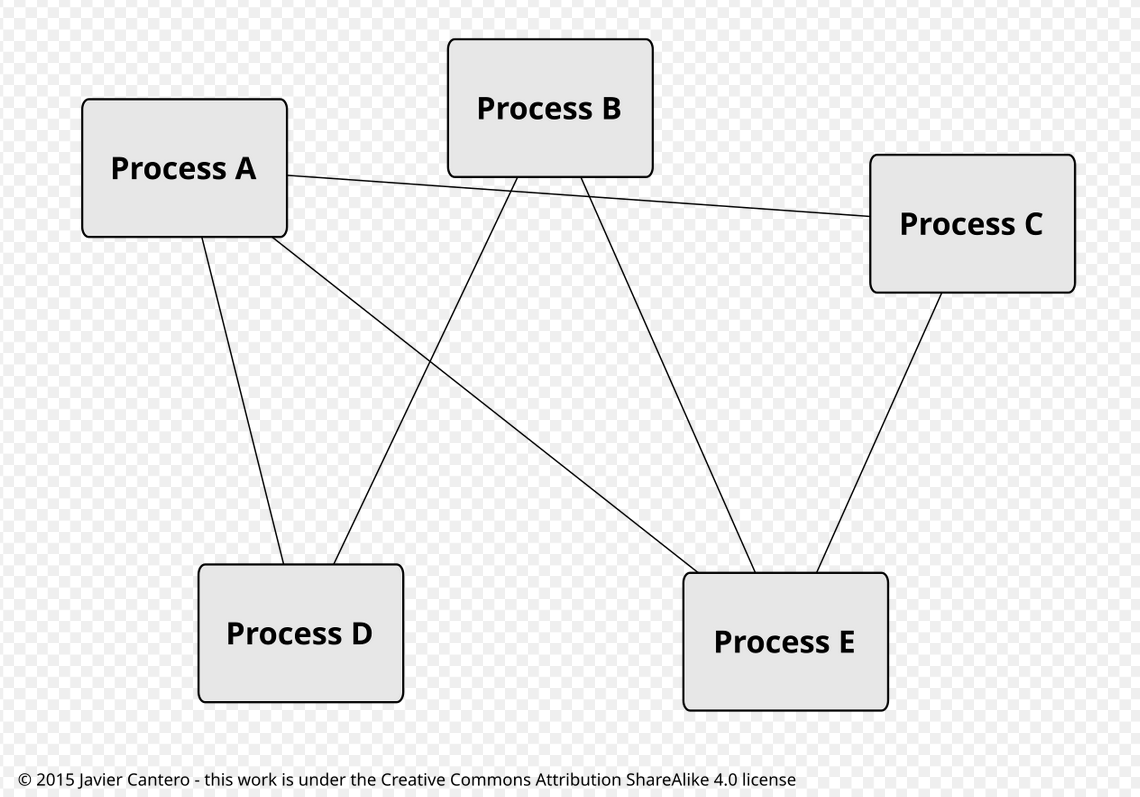
\includegraphics[width=\textwidth,height=\textheight,keepaspectratio]{ipc.png}
\end{frame}

\begin{frame}
    \frametitle{Przykłady}
        \begin{itemize}
        \item Pamięć współdzielona
        \item Sockety
        \item Pipe, named pipe
    \end{itemize}
\end{frame}

\begin{frame}
    \frametitle{Wysokopoziomowe rozwiązania}
    \begin{itemize}
        \item CORBA, Common Object Request Broker Architecture
        \begin{itemize}
            \item Skomplikowany, złożony standard
            \item Transparentność lokacji
            \item Problemy z restrykcyjnym firewallem
            \item Brak planu na standard\pause
        \end{itemize}


        \item DCOP, Desktop COmmunication Protocol
        \begin{itemize}
            \item Daemon, implementacja klient-serwer z traffic directorem
            \item C/C++
            \item Zastępiony przez D-Bus
        \end{itemize}
    \end{itemize}

\end{frame}


\begin{frame}
    \frametitle{freedesktop.org}
    Projekt z 2002 roku zarządzający między innymi:
    \begin{itemize}
        \item PulseAudio
        \item systemd
        \item Wayland
        \item Mesa
    \end{itemize}

\end{frame}

\begin{frame}
    \frametitle{D-Bus}
    Potrzeba zaimplementowania ustandaryzowanego,
    bezpiecznego IPC dla
    środowisk graficznych.

    2002 - początek projektu

    2006 - stabilna wersja
\end{frame}

\begin{frame}
    \frametitle{Zalety}
    \begin{itemize}
        \item Prosty 
        \item Dostępność standardu w wielu językach programowania 
        \item Security policy 
        \item Abstrakcja połączenia 
        \item Walidacja typów
        \item Centralizacja
        \item Działanie ad hoc
    \end{itemize}
\end{frame}